%% -*- coding:utf-8 -*-

\section{Minimalism}

\subtitle{Minimalism}

\huberlintitlepage[22pt]


\outline{

\begin{itemize}
\item Introduction and basic terms
\item Phrase structure grammar and \xbar Theory
\item Government \& Binding (GB)
\item {Generalized Phrase Structure Grammar (GPSG)}
\item {Feature descriptions, feature structures and models}
\item {Lexical Functional Grammar (LFG)}
\item {Categorial Grammar (CG)}
\item Head-Driven Phrase Structure Grammar (HPSG)
\item Tree Adjoning Grammar (TAG)
\end{itemize}

Bonus material:
\begin{itemize}
\item \alert{Minimalism}
\item Construction Grammar (CxG)
\item Dependency Grammar (DG)
\end{itemize}

%\tableofcontents
}



\frame{
\frametitle{Minimalism}


\begin{itemize}
\item developed at the MIT in Boston by Noam Chomsky like GB \citeyearpar{Chomsky93b-u,Chomsky95a-u}
\item Problem of evolution of language: if language specific knowledge is encoded in our genome, how
  did it get there?
\item So: assumed language-specific knowledge should be minimal \citep*{HCF2002a}
 
\item Internationally wide-spread. Independent infrastructure for journals, conferences etc.

\item Germany: 
      \begin{itemize}
      \item Artemis Alexiadou, Humboldt-Universität zu Berlin; 
      \item Günther Grewendorf, Frankfurt am Main; 
      \item Joseph Bayer, Konstanz; 
      \item Gereon Müller, Leipzig.
      \end{itemize}
\end{itemize}
\nocite{Grewendorf2002a}

}

\frame{
\frametitle{Minimalism}


\begin{itemize}
\item GB and \xbar analyses were taken up in many other theories (GPSG, LFG, HPSG, TAG),
  this is less frequently the case for Minimalist analyses.
\item But there are interesting works and the goal of this session is to enable you to read them and
  understand them.

\item Explosion of variants after 1993. 
\begin{itemize}
\item \citet{Kayne94a-u}
\item \citet{Rizzi97a-u}: Cartography
\item \citet{Borer2003a-u,Borer2005a-u}: Exoskeletal approaches
\item \citet{Starke2009a}: Nano syntax
\end{itemize}

I assume the version of \citet{Adger2003a} in what follows.

\item textbooks: \citet*{Adger2003a,Radford97a-u,HNG2005a} (Vorsicht, Haltbarkeitsdatum evtl.\ überschritten)

\item overview articles: \citet{Richards2015a}

\end{itemize}
\nocite{Grewendorf2002a}

}

\subsection{Allgemeines zum Repräsentationsformat}

\frame{
\frametitle{Allgemeines zum Repräsentationsformat}

\begin{itemize}
\item nur zwei Regeln: External Merge und Internal Merge
\item External Merge = Multiplikationsregel der Kategorialgrammatik bzw. Kopf-Komplement-Schema und
  Spezifikator-Kopf Schema der HPSG \citep{BE95a,MuellerUnifying}

\item Internal Merge = Füller-Kopf-Schema der HPSG \citep{MuellerUnifying}

\item Anders als bei CG und HPSG gibt es aber viele, viele Zusatzannahmen.

\end{itemize}

}
\frame{
\frametitle{Architektur}

\begin{itemize}
\item Es gibt keine Tiefenstruktur und Oberflächenstruktur mehr.
\item Kombination und Bewegung sind verwoben.

\medskip

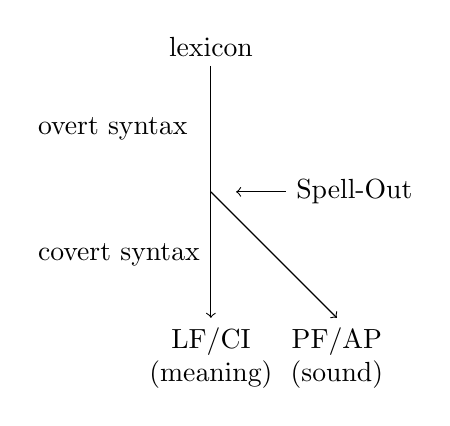
\begin{tikzpicture}[scale=.8]
%\draw (-2.9,-5.8) to[grid with coordinates] (2.7,-0.6);
\draw[->] (0,-1) node[anchor=south] {lexicon} --(0,-5) node[anchor=north, align=center] {LF/CI\\(meaning)};
\draw[->] (0,-3)--(2,-5) node[anchor=north,align=center] {PF/AP\\(sound)};
\draw[<-] (.4,-3)--(1.2,-3) node[anchor=west] {Spell-Out};
%\draw (0,-0.5) node {lexicon};
\draw (-2.9,-2) node[anchor=west] {overt syntax};
\draw (-2.9,-4) node[anchor=west] {covert syntax};
%\draw (0,-6.5) node[align=center] {LF/CI\\(meaning)};
%\draw (2,-5.5) node[align=center] {PF/AP\\(sound)};
\end{tikzpicture}
\end{itemize}

}

\frame{
\frametitle{Phases}

\begin{itemize}
\item Phases: \citet{Chomsky2008a}.
\item Phase is spelled out once it is combined with a head.

\ea
He believes that Peter comes.
\z
\end{itemize}

}


\subsubsection{Valenz, Merkmalsüberprüfung und Agree}
\label{sec-features-minimalism}



\frame{
\frametitle{DP vs.\ NP}


\begin{itemize}
\item Standardannahme im Minimalismus:\\
      \emph{this man} ist eine DP (weil D der Kopf ist, nicht N)

\ea
letters to this man
\z

\pause
\item \emph{him} hat Distribution wie DP, also dieselbe Kategorie:

\ea
letters to him
\z

\end{itemize}
}

\frame{
\frametitle{Valenzrepräsentation über uninterpretierbare Merkmale}


\begin{forest}
baseline
[N 
  [\emph{letters} {[N, pl, \st{\textit{u}P}]}]
  [P
    [\emph{to} {[P, \st{\textit{u}D}]}]
    [\emph{him} {[D]}]]]
\end{forest}

\begin{itemize}
\item \textit{u}D bedeutet, dass ein D gefunden werden muss.
\pause
\item \st{\textit{u}D} bedeutet, dass ein D gefunden wurde.
\end{itemize}

}

\frame{
\frametitle{Valenzrepräsentation und Crash}

\begin{forest}
baseline
[N 
  [\emph{letters} {[N, pl, \st{\textit{u}P}]}]
  [\emph{to} {[P, \textit{u}D]}]]
\end{forest}

\begin{itemize}
\item Objekt ist nicht wohlgeformt, weil \textit{u}D übrig ist.
\item Derivation "`crasht"' an den Interfaces
\end{itemize}

}



\frame[shrink=10]{
\frametitle{Merkmalsüberprüfung mittels Agree}

\eal
\ex[*]{
letters to he
}
\ex[]{
letters to him
}
\zl

\centerline{
\begin{forest}
baseline
[N 
  [\emph{letters} {[N, pl, \st{\textit{u}P}]}]
  [P
    [\emph{to} {[P, \st{\textit{u}D}, \st{acc}]}]
    [\emph{him} {[D, \st{acc}]}]]]
\end{forest}
}

\begin{itemize}
\item Selektionsmerkmale sind atomar, \dash man kann nicht DP[\type{acc}] verlangen.
\item weiterer Mechanismus, der andere Merkmale überprüfen kann: \emph{Agree}
\item über Agree geprüfte Merkmale müssen nicht unbedingt am obersten Knoten präsent sein.
\end{itemize}

}



\subsubsection{Phrasenstruktur und \xbart}

\frame{
\frametitle{Phrasenstruktur und \xbart}

\centerline{
\begin{forest}
%where n children=0{}{},
%sm edges
%for tree={parent anchor=south, child anchor=north,align=center,base=bottom}
[XP
  [specifier]
  [\xbar
    [specifier]
    [\xbar
      [complement] [X] ] ] ]
\end{forest}
}

\begin{itemize}
\item Ob etwas \xbar oder XP ist, hängt davon ab, ob es als Argument benutzt wird oder nicht.
\item vermeidet unschöne unären Verzweigungen der \xbart
\item Probleme: \citew[Abschnitt~2.1]{Brosziewski2003a-u}. 
\end{itemize}

}


\subsubsection{Little \textit{v}}
\label{sec-little-v}

\frame{

\frametitle{Little \textit{v}}

\eal
\ex[*]{
Emily showed himself Benjamin in the mirror.
}
\ex[]{
Peter showed himself Benjamin in the mirror.
}
\zl

\begin{itemize}
\item \emph{himself} kann sich auf Emily, aber nicht auf Benjamin beziehen.

\item \emph{himself} muss höher im Baum sein.
\end{itemize}

}

\frame{
\frametitle{c-command-Anforderungen und ditransitive Verben}

\ea
A node A c-commands B if, and only if A's sister either:\\
\begin{tabular}[t]{@{}l@{~}l@{}}
a. & is B, or\\
b. & contains B
\end{tabular}
\z

\oneline{
\begin{forest}
baseline
[\vbar
 [\textit{show}]
 [\textit{himself}]
 [\textit{Benjamin}]]
\end{forest}
\hfill
\begin{forest}
baseline
[\vbar
   [\vbar
     [\textit{show}]
     [\textit{himself}] ]
 [\textit{Benjamin}]]
\end{forest}
\hfill\hfill
\begin{forest}
baseline
[\littlevbar
 [\textit{show}]
 [VP
   [\textit{himself}]
   [\vbar
    [V]
    [\textit{Benjamin}]]]]
\end{forest}
}
}

\frame{
\frametitle{Ditransitive Verben}

\ea[]{
Peter showed himself Benjamin in the mirror.
}
\z


\begin{itemize}
\item Analyse mit zusätzlichem leeren Verb geht zurück auf \citet{Larson88a}
\item \citet[\page 70]{HK93a-u}: Leeres Verb steuert Kausativsemantik bei.
\item \emph{show} steht in der V-Position und bewegt sich dann zu \textit{v}.
\item \emph{show} bedeutet \emph{see} und bei \littlev kommt dann die kausative Bedeutung dazu,
  woraus sich \relation{cause-see} ergibt \citep[\page 133]{Adger2003a}. 
\end{itemize}

}

\frame{
\frametitle{Ditransitive Verben}
\centerline{
\begin{forest}
baseline
[\vP
  [\textit{Peter}]
  [\littlevbar
   [\textit{v} $+$ \textit{show}]
   [VP
     [\textit{himself}]
     [\vbar
      [\phonliste{ show } {[V]}]
      [\textit{Benjamin}]]]]]
\end{forest}
}
}


\subsubsection{Linking}

\frame{
\frametitle{Little \textit{v} everywhere}

\begin{itemize}
\item Verb-Shell-Analyse ursprünglich nur für ditransitive Verben \citep{Larson88a},\\
 jetzt aber auch für strikt transitive Verben und intransitive Verben verwendet.

\item \citet[Abschnitt~4.5]{Adger2003a}: semantische Rollen einheitlich vergeben:
\eal
\ex DP Tochter von \vP $\to$ interpretiert als agent
\ex DP Tochter von VP $\to$ interpretiert als theme
\ex PP Tochter von \littlevbar $\to$ interpretiert als goal
\zl
\item Adger: einheitlich zugewiesene Rollen helfen bei Spracherwerb,\\
      also \littlev auch bei strikt transitiven und intransitiven Verben.

\item Frage: Involviert \emph{schlafen} eine kausative Komponente? Ein Agens?

\end{itemize}
}

\frame{
\frametitle{Transitive und intransitive Verben}

\vfill
\hfill\begin{forest}
baseline
[\vP
  [Agent]
  [\littlevbar~{[\st{\textit{u}D}]}
   [\textit{v}]
   [VP
      [\textit{burn} {[V, \st{\textit{u}D}]}]
      [Theme]]]]]
\end{forest}
\hfill
\begin{forest}
baseline
[\vP
  [Agent]
  [\littlevbar~{[\st{\textit{u}D}]}
   [\textit{v} ]
   [ \textit{laugh} {[V]} ]]]
\end{forest}
\hfill\mbox{}

\vfill
\begin{itemize}
\item \citet[\page 164]{Adger2003a}:\\
      Auch intransitive und transitive Verben bewegen sich von V nach \textit{v}.
\end{itemize}
\vfill
}

\subsubsection{CP, TP, \vP, VP}
\label{sec-CP-TP-vP-VP}


\subsubsubsection{Merkmale als Auslöser von Bewegungen: Das EPP-Merkmal von T}
\label{sec-epp-features}

\frame{
\frametitle{Merkmale als Auslöser von Bewegung: EPP-Merkmal bei T}

\begin{itemize}
\item In GB waren die Subjekte Spezifikatoren von IP.
\item Jetzt sind sie Spezifikatoren von \vP.
\item Kombiniert man Modalverben mit \vP, steht Subjekt an falscher Stelle.
\eal
\ex[*]{
Will Ann read the book.
}
\ex[]{
Anna will read the book.
}
\zl

\item Annahme eines starken, uninterpretierbaren Merkmals D beim T-Kopf.

\item Starke Merkmale lösen Bewegung aus, weil die Überprüfung lokal erfolgen muss. 
      Sie werden durch ein `*' gekennzeichnet.

\item Da das Merkmal stark ist, muss ein passendes D in die Spezifikatorposition von T bewegt werden
  und das D checken.


\end{itemize}

}

\frame{
\frametitle{Merkmale als Auslöser von Bewegung: EPP-Merkmal bei T}

\centerline{
\scalebox{.8}{%
\begin{forest}
baseline
[TP
 [\textit{Anna} {[D]}]
 [\tbar{[\st{\textit{u}D*}]}
   [\textit{will} T{[pres]}]
   [\vP
     [\phonliste{ Anna }]
     [\littlevbar~{[\st{\textit{u}D}]}
       [\textit{v}
         [\textit{read}] [\textit{v}]]
       [VP
         [\phonliste{ read } {[V, \st{\textit{u}D}]}]
         [DP [\textit{the book}, roof]]]]]]]
\end{forest}
}
}

}

\frame{
\frametitle{EPP: Extended Projection Principle}

\begin{itemize}

\item Das Merkmal wird EPP-Merkmal genannt.\\
      EPP steht für Extended Projection Principle.
\pause

\item EPP gab es schon in der GB: Jeder Satz muss ein Subjekt haben.
\pause

\item Das ist für das Deutsche falsch:
\eal
\ex Mir ist schlecht.
\ex weil noch gearbeitet wurde
\zl

\pause
\item Man kann behaupten, dass in (\mex{0}) leere Subjekte vorliegen,\\das Prinzip wird dadurch aber entwertet.
\end{itemize}
}


\frame{
\frametitle{Komplette Analyse eines Deklarativsatzes mit CP}

\centerline{
\scalebox{.75}{%
\begin{forest}
baseline
[CP
 [C{[Decl]}]
 [TP
 [\textit{Anna} {[D]}]
 [\tbar{[\st{\textit{u}D*}]}
   [\textit{will} T{[pres]}]
   [\vP
     [\phonliste{ Anna }]
     [\littlevbar~{[\st{\textit{u}D}]}
       [\textit{v}
         [\textit{read}] [\textit{v}]]
       [VP
         [\phonliste{ read } {[V, \st{\textit{u}D}]}]
         [DP [\textit{the book}, roof]]]]]]]]
\end{forest}
}
}

}

\frame{
\frametitle{Fragen}

\begin{itemize}
\item Für (\mex{1}) braucht man ein unvalued Satztypen-Merkmal bei T für den Satztyp \emph{question}. 
\ea
What will Anna read?
\z
\item Der leere Komplementierer C hat ein Q-Merkmal, das dem Satztyp-Merkmal bei T einen Wert
  zuweisen kann. (value the feature)
\item Da das Satztypmerkmal bei T strong ist, muss sich das T-Element zu C bewegen, um das Merkmal
  lokal checken zu können.

\item \emph{wh}-Element muss auch bewegt werden. Das wird durch starkes \emph{wh}-Merkmal bei C
  erzwungen.

\end{itemize}

}

\frame{
\frametitle{Fragen: \emph{What will Anna read?}}

\centerline{
\scalebox{.7}{
\begin{forest}
baseline
[CP
 [\textit{what} {[D, wh]}]
 [\cbar{[\st{\textit{u}wh*}]}
   [C
     [\textit{will} T{[\st{Q*}]}]
     [C{[Q]}] ]
   [TP
   [\textit{Anna} {[D]}]
   [\tbar{[\st{\textit{u}D*}]}
     [\phonliste{ will } {[T]}]
     [\vP
       [\phonliste{ Anna }]
       [\littlevbar~{[\st{\textit{u}D}]}
         [\textit{v}
           [\textit{read}] [\textit{v}]]
         [VP
           [\phonliste{ read } {[V, \st{\textit{u}D}]}]
           [\phonliste{what}]]]]]]]]
\end{forest}
}
}
}

\subsubsection{Kasuszuweisung}


\frame{
\frametitle{Kasuszuweisung}

\begin{itemize}
\item Die DPs \emph{Anna} und \emph{the book} haben zu Beginn uninterpretierbare Kasusmerkmale:
[\textit{u}case:]. 
\pause
\item Die Merkmale werden valuiert durch T und \textit{v}.
\pause
\item Nur ein Merkmal wird durch Merge gecheckt. Bei T das D-Merkmal. 
\pause
\item Kasusmerkmal muss mittels eines anderen Checking-Mechanismuses gecheckt werden: Agree.
\pause
\item Agree kann Merkmale in Schwesterknoten checken oder auch weiter weg im Baum.
\pause
\item Knoten muss den Knoten, mit dem es eine Agree-Relation geben soll, c-kommandieren.

\end{itemize}

}

\frame[shrink]{
\frametitle{Kasuszuweisung}

\centerline{
\scalebox{.7}{
\begin{forest}
baseline
[TP
 [\textit{Anna} {[D, \st{nom}]}]
 [\tbar{[\st{\textit{u}D*}, \st{nom}]}
   [T{[pres]}]
   [\vP
     [\phonliste{ Anna }]
     [\littlevbar~{[\st{\textit{u}D}]}
       [\textit{v}
         [\textit{read}] [\textit{v} {[\st{acc}]}]]
       [VP
         [\phonliste{ read } {[V, \st{\textit{u}D}]}]
         [DP{[\st{acc}]} [\textit{the book}, roof]]]]]]]
\end{forest}
}}

\begin{itemize}
\item \textit{v} c-kommandiert VP, V, die DP \emph{the book} und alle Knoten in dieser DP.
\item Da Agree Merkmale von c-kommandierten Knoten valuieren kann,\\
      kann der Akkusativ bei \textit{v} das Kasus-Merkmal der DP \emph{the book} valuen.
\end{itemize}

}


\frame[shrink]{
\frametitle{Nichtlokalität von Agree}

\begin{itemize}
\item Agree kann nicht-lokal Merkmale überprüfen. Aber was ist mit (\mex{1})?
\ea[*]{
\label{ex-him-likes-she}
Him likes she.
}
\z
Der Akkusativ von \textit{v} könnte mit dem Subjekt abgeglichen werden und der Nominativ von T mit
dem Objekt von \emph{likes}.

\centerline{
\scalebox{.7}{
\begin{forest}
baseline
[TP
 [\textit{him} {[D, \st{acc}]}]
 [\tbar{[\st{\textit{u}D*}, \st{nom}]}
   [T{[pres]}]
   [\vP
     [\phonliste{ him }]
     [\littlevbar~{[\st{\textit{u}D},\st{acc}]}
       [\textit{v}
         [\textit{read}] [\textit{v} {[\st{acc}]}]]
       [VP
         [\phonliste{ read } {[V, \st{\textit{u}D}]}]
         [DP{[\st{nom}]} [\textit{she}]]]]]]]
\end{forest}
}}


\end{itemize}
}

\frame{
\frametitle{Nichtlokalität von Agree}

\begin{itemize}
\item Anforderung an Agree: Nimm das nächstmögliche Element.
\item \citet[\page 218]{Adger2003a}:
\ea
\label{principle-locality-of-matching}
Locality of matching\is{locality!of matching}: Agree holds between a feature F on X and a matching feature F on Y if and only
if there is no intervening Z[F].
\z
Intervention ist wie folgt definiert:
\ea
\label{def-intervention}
Intervention\is{intervention}: In a structure [X \ldots{} Z \ldots{} Y], Z intervenes between X and Y iff X
c-commands\is{c"=command} Z and Z c-commands Y.
\z
\item Weil T mit \emph{Anna} Agreen kann, darf es nicht mit \emph{the book} Agreen.
\end{itemize}
}

\subsubsection{Adjunkte}

\frame{
\frametitle{Adjunkte}

\begin{itemize}
\item \citet[Section~4.2.3]{Adger2003a} nimmt an, dass Adjunkte sich mit XP verbinden und eine neue XP
bilden.
\item Er nennt diese Operation \emph{Adjoin}.

\item Operation konsumiert keine Merkmale, ist also anders als External Merge.

\item Das heißt, neue zusätzliche Operation in der Theorie (nicht nur die beiden Merges!).

\item Es gibt Vorschläge, Adjunkte als Elemente innerhalb spezieller adverbieller Phrasen mit leeren
  Köpfen zu behandeln.

\item Ich finde Adgers Lösung besser.\\
      Entspricht dem, was in vielen anderen Frameworks auch gemacht wird.
\end{itemize}

}


\subsection{Verbstellung}
\label{sec-verb-position-MP}

\frame{
\frametitle{Verbstellung}

\begin{itemize}
\item Finites Verb bewegt sich von V zu \textit{v} zu T und dann zu C.
\item Die Bewegung zu T wird durch ein starkes Tense-Merkmal von T erzwungen.
\item Die Bewegung des T-Komplexes nach C wird durch ein Satztypmerkmal ausgelöst, das durch ein
  starkes Interrogativ-Merkmal (Int) bzw. durch ein Deklarativ-Merkmal (Decl) valuiert wird.
\end{itemize}


%% \ea
%% Kennt jeder diesen Roman?
%% \z

}

\frame{
\frametitle{Verbstellung: \emph{Kennt jeder diesen Roman?}}


\scalebox{.7}{
\begin{forest}
[CP
    [C
      [T{[\st{Int*}]}
        [\textit{kennt} {[\st{Pres*}]}]
        [T{[Pres]}]]
      [C{[Int]}]]
    [TP
      [\textit{jeder}]
      [\tbar{[\st{\textit{u}D*}]}
        [\vP
          [\phonliste{ jeder }]
          [\littlevbar
            [VP
              [DP [\textit{diesen Roman}, roof] ]
              [\phonliste{ kennt }]]
            [\textit{v}
              [\phonliste{ kennt }]
              [\textit{v}]]]]
        [\phonliste{ kennt T }]]]]
\end{forest}
}
}


\subsection{Fernabhängigkeiten}

\frame{
\frametitle{Fernabhängigkeiten}

\begin{itemize}
\item Decl bei C löst Verbumstellung aus.
\item Merkmal top löst Bewegung nach SpecCP aus.
\end{itemize}
}

\frame{
\frametitle{Fernabhängigkeiten \emph{Diesen Roman kennt jeder.}}

\scalebox{.7}{
\begin{forest}
[CP
  [\emph{diesen Roman} {[top] }]
  [\cbar{[\st{\textit{u}top*}]}
    [C
      [T{[\st{Decl*}]}
        [\textit{kennt} {[\st{Pres*}]}]
        [T{[Pres]}]]
      [C{[Decl]}]]
    [TP
      [\textit{jeder}]
      [\tbar{[\st{\textit{u}D*}]}
        [\vP
          [\phonliste{ jeder }]
          [\littlevbar
            [VP
              [\phonliste{ diesen Roman }{[D]}]
              [\phonliste{ kennt }]]
            [\textit{v}
              [\phonliste{ kennt }]
              [\textit{v}]]]]
        [\phonliste{ kennt T }]]]]]
\end{forest}
}
}


\subsection{Passiv}

\frame{
\frametitle{Passiv}


\begin{itemize}
\item Wie bei GB weist Verb keinen Akk zu: \littlev hat kein acc-Merkmal.
\item Dafür spezielle Version von \littlev, das auch bei den unakkusativischen Verben eine Rolle spielt \citep{Perlmutter78}.

\citet[\page 140]{Adger2003a}: \vPs für unakkusativische Verben \emph{fall}, \emph{collapse}, \emph{wilt}:

\vfill

\begin{forest}
[\vP
  [\textit{v}]
  [VP
    [\textit{fall}{[V, \textit{u}D]}]
    [Theme]]]
\end{forest}

\vfill

\item Unakkusativisches \littlev spielt auch bei Analyse des Passivs eine Rolle.
\item Es gibt ein Subjekt, das irgendwie Objekteigenschaften hat.
\item Das spezielle \littlev wird von einem Passivkopf \emph{werden} gefordert und\\
      bildet eine Passive Phrase.

\end{itemize}

}

\frame{
\frametitle{Passiv: \emph{dass er geschlagen wurde}}

\centerfit{
%\begin{sideways}  
\begin{forest}
for tree={fit=rectangle}
[TP
     [PassP
       [\vP
         [VP
           [pronoun {[\st{nom}]} ]
           [\phonliste{schlagen}]]
         [\textit{v}
           [\textit{schlagen}]
           [{\textit{v}[\st{\textit{u}Infl}:Pass]}]]]
       [\phonliste{werden}]]
     [{T[past,\st{nom}]}
       [\textit{werden} {[Pass,\st{\textit{u}Infl}:past*]}]
       [{T[past]}]]]
\end{forest}
%\end{sideways}
}

\begin{itemize}
\item Pass-Kopf verlangt Infl-Merkmal von \littlev mit Wert Pass.
\item Partizip-Morphologie bei Spell-Out.
\item Hilfsverb bewegt sich zu T, um starkes Infl zu checken.
\item Weil Infl-Wert past ist, muss Form \emph{wurde} ausgesprochen werden
\item Es gibt keine Bewegung! Kasus wird über Agree vergeben.
\end{itemize}


}

\frame{
\frametitle{Passiv: Aber}

\begin{itemize}
\item Das ist besser als bei der GB-Analyse mit IP.
\item Aber: \citet[\page 332]{Adger2003a} nimmt für Deutsch an, dass es ein starkes EPP-Merkmal
  gibt.
\item Daraus ergeben ich dieselben Probleme wie beim GB-Ansatz.
\item Alle Objekte müssen sich zu T bewegen, auch wenn es keine Umstellung im Satz gibt.
\item Unpersönliche Passive sind problematisch, da es nichts gibt,\\
      was sich zu T bewegen könnte.
\ea
weil getanzt wurde
\z
\end{itemize}
}


\subsection{Lokale Umstellung}

\frame{
\frametitle{Lokale Umstellung}

\begin{itemize}
\item \citet{Adger2003a} behandelt Scrambling nicht.
\item Alle Umordnungen sind merkmalsgesteuert, also muss es irgendein Merkmal geben, das
  Umstellungen wie in (\mex{1}b) auslöst:
\eal
\ex 
{}[weil] jeder diesen Roman kennt
\ex 
{}[weil] diesen Roman jeder kennt
\zl
\item Diverse Vorschläge in der Literatur mit so genannten funktionalen Projektionen:
\begin{itemize}
\item Topic Phrase \citep[\page 222]{Laenzlinger2004a} 
\item AgrS und AgrO \citep[Kapitel~4]{Meinunger2000a}
\end{itemize}
\item Bessere Lösung von G.\ \citet[Abschnitt~3.5]{GMueller2014a-u}:
      Objekt bewegt sich zu zweiter Spezifikatorposition von \littlev. 
\item Dazu werden optionale Merkmale bei \textit{v} und V angenommen (S.\,48).
\end{itemize}
} 

\frame{
\frametitle{Lokale Umstellung \emph{dass diesen Roman jeder kennt}}

\scalebox{.8}{
\begin{forest}
[CP
    [C
      [dass]]
    [TP
        [\vP
          [\emph{diesen Roman}]
          [\littlevbar
            [ \emph{jeder}]
            [\littlevbar
                [VP
                  [\phonliste{ diesen Roman } {[D]}] 
                  [\phonliste{ kennt }]]
                [\textit{v}
                  [\phonliste{ kennt }]
                  [\textit{v}]]]] ]
        [\textit{kennt} {[T]}]]]
\end{forest}
}

}

\frame{
\frametitle{Überblick über Stipulationen}

\begin{itemize}
\item Annahmen in Adgers Analyse:
\begin{itemize}
\item Kategorie eines Knotens hängt davon ab, wie er verwendet wird (noch erweitert oder nicht).
\item Bei Merge kann immer genau ein Merkmal überprüft werden.
\item Andere Merkmale werden mit Agree überprüft.
\item Agree kann Merkmale überprüfen, wenn c-Kommando vorliegt.
\item Agree kann nur dann Merkmale überprüfen, wenn kein anderes Merkmal interveniert.
\item Es gibt starke und schwache Merkmale.
\item Derivationen, die noch Merkmale übrig haben, crashen an den Interfaces.
\end{itemize}
\pause
\item Es gibt ein Spracherwerbsproblem.
\pause
\item Zum Vergleich CG und HPSG:
\begin{itemize}
\item Es gibt einen Funktor mit einer Beschreibung des abhängigen Elements.
\item Abhängiges Element muss passen.
\end{itemize}
\pause
\item Adgers Analyse ist die MP-Analyse mit den wenigsten Stipulationen.
\end{itemize}


}

\subsection{Varianten und Argumentation für Theorien}

\frame{
\frametitle{Varianten und Argumentation für Theorien}

\begin{itemize}
\item Es gibt viele Varianten und Sub-Schulen.
\item Kartographie (Crypto-Konstruktivismus): Probleme mit der Syntax-Semantik-Trennung werden durch
  Syntaktifizierung der Semantik umgangen \citep{Rizzi2014a}
\item Kaynesche Ansätze mit zugrundeliegender Specifier-Head-Complement-Anordnung für alle Sprachen.
\item \ldots
\end{itemize}


}

\frame{
\frametitle{Varianten: \citet{Rizzi97a-u}}

\scalebox{.5}{%
\newlength\mytextheight
\settototalheight{\mytextheight}{XpX$^0$X$'$}
\begin{forest}
  delay={
    where content={}{
      content={\phantom{X}}
    }{},
  },
  for tree={
    text height=\mytextheight,
    fit=band,
    parent anchor=south,
    child anchor=north,
  }
[ForceP
	[]
	[Force$'$
		[Force$^0$]
		[TopP*
			[]
			[Top$'$
				[Top$^0$]
				[FocP
					[]
					[Foc$'$
						[Foc$^0$]
						[TopP*
							[]
							[Top$'$
								[Top$^0$]
								[FinP
									[]
									[Fin$'$
										[Fin$^0$]
										[IP]]]]]]]]]]]
\end{forest}
}

}


\frame{
\frametitle{Evidence from a single language and UG}


\begin{itemize}
\item What does it mean for other languages\\
      that a rule/morpheme is present in one particular language?
\pause
\item Possible answer:\\
      If we have a certain structure in language X,\\
      it must be present in all languages.
\pause
\item Example:
      \begin{itemize}
      \item Basque: Tree positions for object agreement (AgrO, AgrIO)\nocite{Chomsky93b-u,Stechow96a,Grewendorf2002a,Meinunger2000a}
      \item Japanese/Gungbe: Tree position for topic marker\nocite{CR2010a} %\citet[\page 62]{CR2010a}
      \end{itemize}

\pause
\item German and Dutch neither have object agreement nor topic morphemes.

\pause
\item Conclusion:\\
      If such inferences regarding properties of particular languages are made,\\
      one has to assume (very specific!) innate linguistic knowledge.

\end{itemize}

% Parameter
\nocite{Newmeyer2005a}
}

%% \frame[shrink]{
%% \frametitle{AgrS, AgrIO und AgrO nach \citew[S.\,101]{Meinunger2000a}}

%% \begin{columns}[T]

%% \begin{column}{65mm}
%% \scalebox{0.4}{\begin{pspicture}(1.6,0)(17.4,16.3)
%% %\psgrid
%% %% \only<handout>{\psline[linewidth=5mm,linecolor=red](3,14)(16,1)
%% %% \psline[linewidth=5mm,linecolor=red](3,1)(16,14)}
%% \rput[B](3,0){\rnode{die Firma}{die Firma Müller}}
%% \rput[B](6,0){\rnode{meinem Onkel}{meinem Onkel}}
%% \rput[B](9,0){\rnode{diese Moebel}{diese Möbel}}
%% \rput[B](12,0){\rnode{erst gestern}{erst gestern}}
%% \rput[B](15,0){\rnode{zugestellt}{zugestellt}}
%% \rput[B](17,0){\rnode{hat}{hat}}
%% %
%% \rput[B](14,2){\rnode{tdo}{t\sub{DO}}}
%% \rput[B](15,2){\rnode{v}{V}}
%% \rput[B](14.5,3){\rnode{vp1}{VP}}
%% %
%% \rput[B](13.5,3){\rnode{tio}{t\sub{IO}}}
%% \rput[B](14,4){\rnode{vs}{V'}}
%% %
%% \rput[B](13,4){\rnode{tsu}{t\sub{SU}}}
%% \rput[B](13.5,5){\rnode{vp2}{VP}}
%% %
%% \rput[B](12,5){\rnode{adv}{Adv}}
%% \rput[B](13,6){\rnode{vp3}{VP}}
%% %
%% \rput[B](15,6){\rnode{agro0}{AgrO$^0$}}
%% \rput[B](14,7){\rnode{agros}{AgrO'}}
%% %
%% \rput[B](9,7){\rnode{do}{DO}}
%% \rput[B](11.5,9){\rnode{agrop}{AgrOP}}
%% %
%% \rput[B](13.5,9){\rnode{agrio0}{AgrIO$^0$}}
%% \rput[B](12.5,10){\rnode{agrios}{AgrIO'}}
%% %
%% \rput[B](6,10){\rnode{io}{IO}}
%% \rput[B](9.25,12){\rnode{agriop}{AgrIOP}}
%% %
%% \rput[B](17,12){\rnode{agrs0}{AgrS$^0$}}
%% \rput[B](13.125,14){\rnode{agrss}{AgrS'}}
%% %
%% \rput[B](3,14){\rnode{su}{SU}}
%% \rput[B](8.06125,16){\rnode{agrsp}{AgrSP}}
%% %
%% \psset{angleA=-90,angleB=90,arm=0pt}
%% %
%% \ncdiag{vp1}{v}
%% \ncdiag{vp1}{tdo}
%% %
%% \ncdiag{vs}{tio}
%% \ncdiag{vs}{vp1}
%% %
%% \ncdiag{vp2}{vs}
%% \ncdiag{vp2}{tsu}
%% %
%% \ncdiag{vp3}{vp2}
%% \ncdiag{vp3}{adv}
%% %
%% \ncdiag{agros}{vp3}
%% \ncdiag{agros}{agro0}
%% %
%% \ncdiag{agrop}{agros}
%% \ncdiag{agrop}{do}
%% %
%% \ncdiag{agrios}{agrop}
%% \ncdiag{agrios}{agrio0}
%% %
%% \ncdiag{agriop}{agrios}
%% \ncdiag{agriop}{io}
%% %
%% \ncdiag{agrss}{agriop}
%% \ncdiag{agrss}{agrs0}
%% %
%% \ncdiag{agrsp}{agrss}
%% \ncdiag{agrsp}{su}
%% %
%% \pstriangle(3,0.4)(2.6,13.5)
%% \pstriangle(6,0.4)(2.3,9.5)
%% \pstriangle(9,0.4)(1.9,6.5)
%% \pstriangle(12,0.4)(1.7,4.5)
%% \ncdiag{v}{zugestellt}
%% \ncdiag{agrs0}{hat}
%% %% \only<beamer>{\only<3->{\psline[linewidth=5mm,linecolor=red](3,14)(16,1)
%% %% \psline[linewidth=5mm,linecolor=red](3,1)(16,14)}}
%% \end{pspicture}}
%% \end{column}
%% \begin{column}{55mm}
%% {\footnotesize
%% \begin{itemize}
%% \item Objektkongruenz im Baskischen.

%%       Wir modellieren das mit Baumkonfigurationen. $\to$

%%       Es muss die Konfigurationen in allen Sprachen geben.
%% \pause
%% \item Wenn wir den Baum schon mal haben, können
%%       wir ihn für die Modellierung d.\ Informationsstruktur im Deutschen benutzen.
%% \pause
%% \item Nein! Kongruenz ist eine Eigenschaft der beteiligten Objekte:\\
%%       die Gleichheit von Werten.

%%       Konfigurationale Aspekte sind dabei irrelevant.
%% \end{itemize}
%% }
%% \end{column}
%% \end{columns}

%% }



\frame{
\frametitlefit{Deutsch ist Englisch/Romanisch (SVO, Laenzlinger nach Kayne)}

\nocite{Laenzlinger2004a,Kayne94a-u}
\begin{columns}[T]

\begin{column}{80mm}
\mode<beamer>{%
\scalebox{0.5}{
\small
\psset{xunit=10mm,yunit=6mm}
%
\begin{pspicture}(-0.4,3)(16.2,20.8)
\rput[B](2,20){\rnode{CP}{CP}}
\rput[B](0,18){\rnode{C}{\cnull}}
\rput[B](4,18){\rnode{SubjP}{SubjP}}
\rput[B](2,16){\rnode{SpecSubjP}{\alt<32->{DP}{XP}}}
\rput[B](6,16){\rnode{ObjP}{\ldots ObjP}}
\rput[B](4,14){\rnode{SpecObjP}{\alt<15->{DP}{XP}}}
\rput[B](8,14){\rnode{AuxP}{\ldots AuxP}}
\rput[B](6,12){\rnode{SpecAuxP}{\alt<49->{VP}{XP}}}
\rput[B](10,12){\rnode{AuxPlus}{Aux+}}
\rput[B](8,10){\rnode{Aux}{Aux}}
\rput[B](12,10){\rnode{vP}{$\nu$P}}
\rput[B](10,8){\rnode{SpecvP}{DP}}
\rput[B](14,8){\rnode{VP}{VP}}
\rput[B](12,6){\rnode{V}{\visible<beamer| beamer:-36>{V}}}
\rput[B](16,6){\rnode{ObjDP}{\visible<beamer| beamer:-36>{DP}}}
%
\psset{angleA=-90,angleB=90,arm=0pt}
%
\ncdiag{CP}{C}\ncdiag{CP}{SubjP}
\ncdiag{SubjP}{SpecSubjP}\ncdiag{SubjP}{ObjP}
\ncdiag{ObjP}{SpecObjP}\ncdiag{ObjP}{AuxP}
\ncdiag{AuxP}{SpecAuxP}\ncdiag{AuxP}{AuxPlus}
\ncdiag{AuxPlus}{Aux}\ncdiag{AuxPlus}{vP}
\ncdiag{vP}{SpecvP}\ncdiag{vP}{VP}
%
\rput[B](0,4){\rnode{weil}{weil}}
\rput[B](2,4){\rnode{er-vorn}{\visible<beamer| beamer:-32>{[ \_ ]}}}
\rput[B](4,4){\rnode{ihn-vorn}{\visible<beamer| beamer:-15>{[ \_ ]}}}
\rput[B](6,4){\rnode{gelesen-vorn}{\visible<beamer| beamer:-49>{[ \_ ]}}}
\rput[B](8,4){\rnode{hat}{hat}}
\rput[B](10,4){\rnode{er}{\visible<beamer| beamer:-18>{er}}}
\rput[B](12,4){\rnode{gelesen}{\visible<beamer| beamer:-35>{gelesen}}}
\rput[B](14,4){\rnode{trace-VP}{\visible<beamer| beamer:37->{[ \_ ]$_k$}}}
\rput[B](16,4){\rnode{ihn}{\visible<beamer| beamer:1>{ihn$_j$}}}
%
\ncdiag{C}{weil}
\ncdiag{SpecSubjP}{er-vorn}
\ncdiag{SpecObjP}{ihn-vorn}
\visible<beamer| beamer:-49>{\ncdiag{SpecAuxP}{gelesen-vorn}}
\ncdiag{Aux}{hat}
\ncdiag{SpecvP}{er}

\alt<-36>{
\ncdiag{VP}{V}\ncdiag{VP}{ObjDP}
\ncdiag{V}{gelesen}
\ncdiag{ObjDP}{ihn}
}{
\ncdiag{VP}{trace-VP}
}

\visible<beamer| beamer:50->{\pstriangle(6,4.6)(2,7.2)}
%\pscircle(12,8.5){1.9}
%\psline{->}(12,5.4)(12,5)(6,5)(6,5.6)
%\psline{->}(14,7.8)(14,4)(4,4)(4,5.6)
% 16 * .75 = 12
%  4 * .6  = 2.4
%
% 10 * .75 = 7.5 
%  2 * .75 = 1.5
\tmove<2-17>(16cm,2.4cm)(4cm,2.4cm){ihn$_j$}{\visible<beamer| beamer:-36>{[ \_ ]$_j$}}
\tmove<19-34>(10cm,2.4cm)(2cm,2.4cm){er$_i$}{[ \_ ]$_i$}
% The whole VP is the trace.
\tmove<36-51>(12cm,2.4cm)(6cm,2.4cm){[gelesen [ \_ ]$_j$ ]$_k$}{}
%\psgrid
%
\end{pspicture}
}
}
\mode<handout>{%
\scalebox{0.5}{
\small
\psset{xunit=9mm,yunit=6mm}
%
\begin{pspicture}(-0.4,1)(16.2,20.8)
\rput[B](2,20){\rnode{CP}{CP}}
\rput[B](0,18){\rnode{C}{\cnull}}
\rput[B](4,18){\rnode{SubjP}{SubjP}}
\rput[B](2,16){\rnode{SpecSubjP}{DP}}
\rput[B](6,16){\rnode{ObjP}{\ldots ObjP}}
\rput[B](4,14){\rnode{SpecObjP}{DP}}
\rput[B](8,14){\rnode{AuxP}{\ldots AuxP}}
\rput[B](6,12){\rnode{SpecAuxP}{VP}}
\rput[B](10,12){\rnode{AuxPlus}{Aux+}}
\rput[B](8,10){\rnode{Aux}{Aux}}
\rput[B](12,10){\rnode{vP}{$\nu$P}}
\rput[B](10,8){\rnode{SpecvP}{DP}}
\rput[B](14,8){\rnode{VP}{VP}}
\rput[B](12,6){\rnode{V}{{V}}}
\rput[B](16,6){\rnode{ObjDP}{{DP}}}
%
\psset{angleA=-90,angleB=90,arm=0pt}
%
\ncdiag{CP}{C}\ncdiag{CP}{SubjP}
\ncdiag{SubjP}{SpecSubjP}\ncdiag{SubjP}{ObjP}
\ncdiag{ObjP}{SpecObjP}\ncdiag{ObjP}{AuxP}
\ncdiag{AuxP}{SpecAuxP}\ncdiag{AuxP}{AuxPlus}
\ncdiag{AuxPlus}{Aux}\ncdiag{AuxPlus}{vP}
\ncdiag{vP}{SpecvP}\ncdiag{vP}{VP}
%
\rput[B](0,4){\rnode{weil}{weil}}
\rput[B](2,4){\rnode{er-vorn}{er}}
\rput[B](4,4){\rnode{ihn-vorn}{ihn}}
\rput[B](6,4){\rnode{gelesen-vorn}{gelesen}}
\rput[B](8,4){\rnode{hat}{hat}}
%\rput[B](10,4){\rnode{er}{\visible<beamer| beamer:-18>{er}}}
%\rput[B](12,4){\rnode{gelesen}{\visible<beamer| beamer:-35>{gelesen}}}
%\rput[B](14,4){\rnode{trace-VP}{\visible<beamer| beamer:37->{[ \_ ]$_k$}}}
%\rput[B](16,4){\rnode{ihn}{\visible<beamer| beamer:1>{ihn$_j$}}}
%
\ncdiag{C}{weil}
\ncdiag{SpecSubjP}{er-vorn}
\ncdiag{SpecObjP}{ihn-vorn}
\ncdiag{SpecAuxP}{gelesen-vorn}
\ncdiag{Aux}{hat}
\ncdiag{SpecvP}{er}

\ncdiag{VP}{V}\ncdiag{VP}{ObjDP}
\ncdiag{V}{gelesen}
\ncdiag{ObjDP}{ihn}

\visible<beamer| beamer:50->{\pstriangle(6,4.6)(2,7.2)}
\pscircle(14,6.5){2.3}
\psline{->}(10,7.8)(10,3)(2,3)(2,3.6)
\psline{->}(14,2.6)(14,2)(6,2)(6,3.6)
\psline{->}(16,5.8)(16,1)(4,1)(4,3.6)
%\psgrid
%
\end{pspicture}
}
}
\end{column}
\begin{column}{40mm}
\footnotesize
\begin{itemize}
\item All languages are Spr-H-Comp underlyingly.
\item<2-> The object is moved out of the VP.
\item<19-> The subject is fronted.
\item<36-> The empty VP is fronted.
\item<52-> There are further empty heads \citep{Cinque99a-u}.
\item<53-> Innateness has to be assumed.
\end{itemize}
\end{column}
\end{columns}

\pause
\pause
\pause
\pause
\only<54>{}


\nocite{Haider2000a}
% against remnant movement
\nocite{Fanselow2002a}


}


\frame{
\frametitle{Deutsch ist Deutsch (GB-Varianten, CG, LFG, HPSG, \ldots)}


\centerline{%
\begin{forest}
sm edges
[CP
 [C [weil]]
 [VP
   [NP [er]]
   [V$'$
     [NP [ihn]]
     [V
       [V [gelesen]]
       [V [hat]]]]]]
\end{forest}
\hfill
\begin{forest}
sm edges
[CP
 [C [weil]]
 [VP
   [NP [er]]
   [NP [ihn]]
   [V [gelesen]]
   [V [hat]]]]
\end{forest}
}

\nocite{Fanselow2001a,CJ2005a,BvN98a}

}

%\fi

\frame{
\frametitle{English, German, \ldots{} are Hungarian}
\begin{columns}[T]

\begin{column}{35mm}
\scalebox{0.65}{
\psset{xunit=5mm,yunit=5mm}
\begin{pspicture}(-1.6,0)(8.6,11)
\rput[B](1.5,10){\rnode{AgrP}{\alert<beamer| beamer:1>{AgrP}}}
\rput[B](-1,8){\rnode{SpecAgrP}{\alt<34->{DP}{XP}}}
\rput[B](-1,0){\rnode{mir}{\visible<beamer| beamer:35->{mir$_j$}}}
\rput[B](4,8){\rnode{Agrs}{\alert<beamer| beamer:1>{Agr$'$}}}
\rput[B](2,6){\rnode{Agr}{\alert<beamer| beamer:1>{Agr}}}
\rput[B](2,0){\rnode{Agrw}{\visible<beamer| beamer:-14>{\trace}}}
\rput[B](6,6){\rnode{PP}{PP}}
\rput[B](6,4){\rnode{Ps}{P$'$}}
\rput[B](4,2){\rnode{P}{P}}
\rput[B](4,0){\rnode{in}{\visible<beamer| beamer:-1>{hinter}}}
\rput[B](8,2){\rnode{DP}{DP}}
\rput[B](8,0){\rnode{dS}{\visible<beamer| beamer:-19>{mir}}}
%
\psset{angleA=-90,angleB=90,arm=0pt}
%
\alert<1>{\ncdiag{AgrP}{SpecAgrP}\ncdiag{AgrP}{Agrs}%
\ncdiag{Agrs}{Agr}\ncdiag{Agrs}{PP}%
\ncdiag{Agr}{Agrw}}%
\ncdiag{PP}{Ps}%
\ncdiag{Ps}{P}\ncdiag{Ps}{DP}%
\ncdiag{P}{in}
\ncdiag{DP}{dS}
\visible<33->{\ncdiag{SpecAgrP}{mir}}
%\psgrid
\tmove<2-17>(2cm,0cm)(1cm,0cm){hinter$_i$}{\trace$_i$}
\tmove<19-34>(4cm,0cm)(-0.5cm,0cm){mir$_j$}{\trace$_j$}
\end{pspicture}

}
\end{column}
\begin{column}{85mm}
\begin{itemize}
\item<1-> \citet*[p.\,124]{HNG2005a}: agreement head for the checking of case features
\item<2-> Preposition is moved there.
\item<19-> DP is put into the specifier position of this head.
\item<36-> Evidence for this:\\ Agreement in Hungarian postpositional phrases
\item<37-> English is like Hungarian,\\
      but the movement is invisible.
\end{itemize}
\end{column}
\end{columns}
}


%\if 0
\frame{
\frametitle{Deutsch ist Deutsch, \ldots{} Ungarisch ist Ungarisch}

\begin{columns}[T]

\begin{column}{35mm}
\scalebox{0.7}{
\psset{xunit=5mm,yunit=5mm}
\begin{pspicture}(-1,0)(4.6,5)
\rput[B](2,4){\rnode{PP}{PP}}
\rput[B](0,2){\rnode{P}{P}}
\rput[B](4,2){\rnode{DP}{DP}}
\rput[B](0,0){\rnode{hinter}{hinter}}
\rput[B](4,0){\rnode{mir}{mir}}
%
\psset{angleA=-90,angleB=90,arm=0pt}
%
\ncdiag{PP}{P}\ncdiag{PP}{DP}
\ncdiag{P}{hinter}\ncdiag{DP}{mir}
%\psgrid
\end{pspicture}
}
\end{column}
\begin{column}{85mm}
\begin{itemize}[<+->]
\item A PP is a P together with an NP (or DP).
\item No movement instead of two movements.
\item Structure has five nodes less.
\item Truly minimal!
\item Question: What constitutes an explanation?\\
      Where and how is complexity of language represented?
\end{itemize}
\end{column}
\end{columns}


}


\frame{
\frametitle{Der Schweizer Käse}

\begin{columns}[T]
\begin{column}{55mm}
\scalebox{.8}{%
\begin{forest}
sm edges without translation
[pP
   [p
	[P [with]]
	[p [$\varnothing$]]]
   [AgrOP
	[D [\textbf{me}]]
	[$\overline{\mbox{AgrO}}$
		[AgrO
			[P [t$'$]]
			[AgrO [,phantom  ]]]
		[PP
			[P [t]]
			[D [\textbf{t}]]]]]]
\end{forest}}
\end{column}
\begin{column}{65mm}
\begin{itemize}
\item from another text book:\\
      \citet[\page 452]{Radford97a-u}
\item \citet[\page 549--550]{Sternefeld2006a-u} calls this a Swiss Cheese analysis, but there are more holes (5) than cheese (2).
\end{itemize}
\end{column}
\end{columns}
}


\subsection{Fundamentale Probleme}

\frame{
\frametitle{Fundamentale Probleme: Kopflose Strukturen}


\begin{itemize}
\item Annahme: Es gibt immer einen Kopf und Strukturen sind binär.
\item Problematisch sind NPN-Konstruktionen \citep{Jackendoff2008a,Bargmann2015a,MuellerCxG}:

\eal
\ex Student after student left the room.
\ex
\label{ex-npn-iteration}
Day after day after day went by, but I never found the courage to talk to
her. \citep{Bargmann2015a}
\zl

\item Jackendoff: 
\begin{itemize}
\item Weder N noch P kann sinnvoll als Kopf bezeichnet werden. 
\item \xbart nicht anwendbar.
\item Semantik nicht kompositional.
\end{itemize}

\end{itemize}



}


\frame{
\frametitle{Fundamentale Probleme: Kopflose Strukturen}


\begin{itemize}

\item G.\,\citet{GMueller2011a} schlägt vor, NPN als Reduplikation zu analysieren: Besondere Form der
  Präposition löst Verdopplung aus.

\item Behauptung: Im Deutschen gäbe es keine NPN-Konstruktionen mit Adjektiven. Ist falsch:
\ea
Die beiden tauchten nämlich geradewegs wieder aus dem heimischen Legoland auf, wo sie im
Wohnzimmer, schwarzen Stein um schwarzen Stein, vermeintliche Schusswaffen nachgebaut
hatten.\footnote{
  taz, 05.09.2018, S.\,20
}
\z
\item Außerdem funktioniert Reduplikation nicht für Iteration wie in (\mex{1}).
\ea
Day after day after day went by, but I never found the courage to talk to
her. \citep{Bargmann2015a}
\z


\end{itemize}



}

%      <!-- Local IspellDict: en_US-w_accents -->
